\documentclass[border=0.2cm]{standalone} 
\usepackage[pdftex]{graphicx}
\usepackage{tikz}
\usetikzlibrary{decorations.pathmorphing,patterns}
\usepackage{xcolor}
\usepackage{pdflscape}

%Set style fo dashed lines
\tikzset{%
  my dash pattern/.style = {
    dash pattern = {on 10pt off 2pt},
  }
}

\begin{document}


\centering
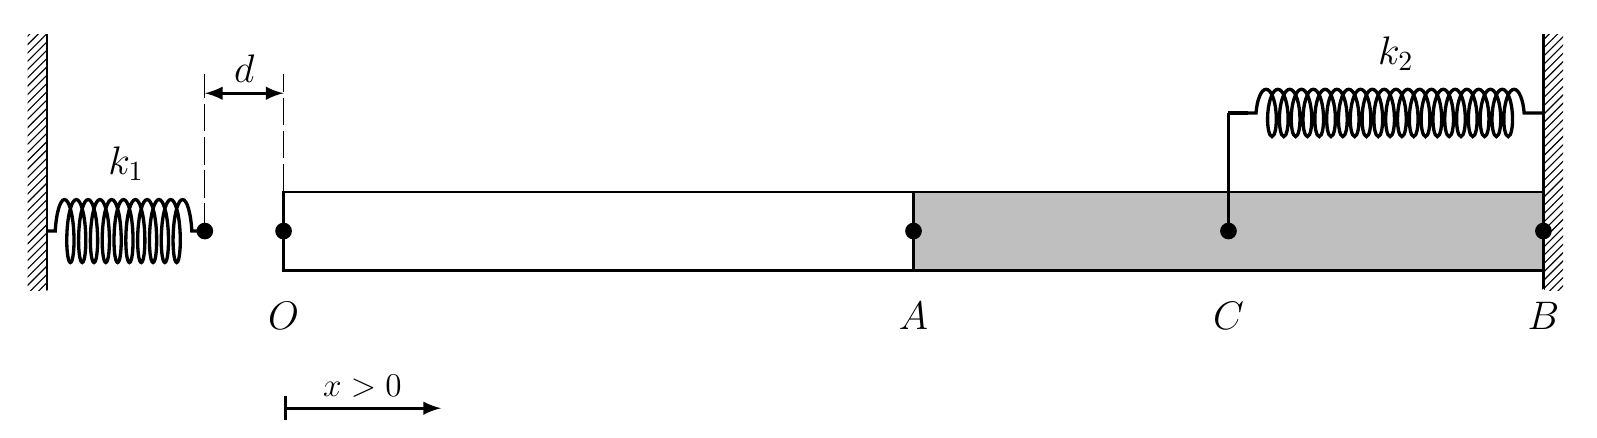
\begin{tikzpicture}
\draw[very thick, decoration={aspect=0.2, segment length=1.5mm,
  amplitude=4mm,post length = 1mm, pre length = 1mm, 
  coil},decorate] (-3,0) -- (-1,0) node[midway,above=0.5cm,black]{\Large
  $k_{1}$}; 
\draw[very thick, decoration={aspect=0.3, segment length=1.5mm,
  amplitude=3mm, pre length = 1mm, post length = 1mm, 
  coil},decorate] (12.25,1.5) -- (16,1.5) node[midway,above=0.4cm,black]{\Large
  $k_{2}$};
\fill [thick,pattern = north east lines] (-3.25,-0.75) rectangle (-3.0,2.5);
\draw[thick] (-3.0,-0.75) -- (-3.0,2.5);%\pszigzag[coilheight=0.3](-4,0)(-2,0);
\draw [thick,fill = white] (0.0,-0.5) rectangle (8.0,0.5); 
\draw [thick,fill = lightgray] (8.0,-0.5) rectangle (16.0,0.5); 
\draw [thick] (16,-0.75) -- (16,2.5);
\fill [thick, pattern = north east lines] (16,-0.75) rectangle (16.25,2.5);
\draw [very thick] (12,1.5) -- (12.25,1.5);
\draw [very thick] (12,0) -- (12, 1.5);
 \node[circle,fill=black,inner sep=0.75mm] (L) at (-1,0) {};
 \node[circle,fill=black,inner sep=0.75mm] (O) at (0,0) {};
 \node[circle,fill=white,inner sep=0.00mm,label=south:\Large $O$] (o) at (0,-0.75) {};
 \node[circle,fill=black,inner sep=0.75mm] (A) at (8,0) {};
 \node[circle,fill=white,inner sep=0.00mm,label=south:\Large $A$] (a) at (8,-0.75) {};
 \node[circle,fill=black,inner sep=0.75mm] (C) at (12,0) {};
 \node[circle,fill=white,inner sep=0.00mm,label=south:\Large $C$] (c) at (12,-0.75) {};
 \node[circle,fill=black,inner sep=0.75mm] (B) at (16,0) {};
 \node[circle,fill=white,inner sep=0.00mm,label=south:\Large $B$] (b) at (16,-0.75) {};
\draw[my dash pattern] (-1,0) -- (-1,2);
\draw[my dash pattern] (0,0.5) -- (0,2); 
\draw[latex-latex,very thick] (-1,1.75) --
  (0.0,1.75)node[midway,above]{\Large $d$};
\draw[very thick,
    black,
    |-latex] (0,-2.25) -- ++(2,0)
    node[midway,above]{\large $x > 0$};
\end{tikzpicture}
\end{document}


